\documentclass{tufte-handout}

%\geometry{showframe}% for debugging purposes -- displays the margins
\usepackage{hyperref}
\hypersetup{colorlinks = true, linkcolor = blue, urlcolor = blue}
\usepackage{amsmath}

% Set up the images/graphics package
\usepackage{graphicx}
\setkeys{Gin}{width=\linewidth,totalheight=\textheight,keepaspectratio}
\graphicspath{{graphs/}}

\title{Evaluating Round 1 Pairing through Simulation%
%\vspace{0.06in} \Large{Analytics Subcommittee}%
%\thanks{Annie J. Wang, Mike Nelson, Ben Graham}
}
\author{Analytics Subcommittee}
%\date{24 January 2009}  % if the \date{} command is left out, the current date will be used

% The following package makes prettier tables.  We're all about the bling!
\usepackage{booktabs}

% The units package provides nice, non-stacked fractions and better spacing
% for units.
\usepackage{units}

% The fancyvrb package lets us customize the formatting of verbatim
% environments.  We use a slightly smaller font.
\usepackage{fancyvrb}
\fvset{fontsize=\normalsize}

% Small sections of multiple columns
\usepackage{multicol}

\begin{document}

\maketitle

\begin{abstract}
\noindent We describe how simulations can help evaluate 
changes to tabulation structure and explore an application to Round 1 pairing. Our results show that random pairings outperforms alternative procedures such as power-matching, folding, and a combination of the two.
\end{abstract}

%\printclassoptions

\section{Why Simulate}
What is the best way to evaluate changes in tabulation procedure?

Every year, the American Mock Trial Association (AMTA) receives numerous motions to change aspects of its tabulation procedure, yet the AMTA Board of Directors lacks a standard methodology to evaluate the impact of these changes. Indeed, this type of analysis can be extremely challenging since, ideally, it entails a near-impossible task: to observe simultaneously how a tournament (or series of tournaments) would play out with and without the proposed change. %\marginnote{In this social sciences, this is called fundamental problem of causal inference: it is impossible to observe the outcome of the same subject with and without some given treatment.}
Historically, motions dealing with tabulation procedure are supported by anecdotal evidence from previous tournaments or informal models of tournament progression. However, these approaches are unsatisfying solutions to this problem of simultaneous observation. Anecdotal evidence often relies on speculative leaps to describe the impact of changes on specific instances and entirely fails to capture the generalized impact of changes. Even when arguments in favor of a proposal are more abstract, they are rarely sufficiently formalized to capture the complete impact of the change and the expected decrease in error.

In response to these problems, we propose that AMTA test structural changes through simulation. Broadly speaking, simulations are simplified models of a real-world process (in this case, mock trial tournaments). The simulator specifies both the procedural rules of the simulation (e.g., tabulation rules) as well as the initial inputs (e.g., the number of teams and the distribution of their `true strength'), and after repeating this process many times, estimates the impact of changing particular features of the simulation.

We believe that simulations are superior to existing methods of evaluating changes to tabulation structure for three reasons. First, evaluations can specify a common set of starting points for parallel simulations, which can be used to test variations in the procedural rules (e.g., using the same set of 24 teams, we can see which of two different pairing systems more accurately captures the true ordering). Second, simulation results can precisely measure the degree to which a proposed change improves (or fails to improve) some outcome (e.g., ranking accuracy). Third, the data generated by simulations offers unprecedented detail into impacts of any changes and how sensitive they are to any inputs (e.g., the distribution of team strength). 

\section{Round 1 Pairing Procedures}

According to the AMTA tabulation manual, the first round of an AMTA-sanctioned tournament is paired at random.\marginnote{CITE.
%Many invitational tournaments have introduced variations to Round 1 pairings, the most common of which `challenge order'. Teams are first ranked according to strength (in practice, this is often measured by performance at the prior year's tournament or using BBR), and starting with the top-ranked team, each team select any team ranked beneath them to compete in Round 1 until all teams have been assigned an opponent.
} Over the last two years, members of the AMTA community have proposed various changes to Round 1 pairing procedures, none of which have been adopted by the AMTA Board of Directors. As a demonstration of the use of simulations, we test and analyze the impact of various Round 1 pairing procedures, including but not limited to those proposed to the AMTA board. Below, we briefly describe the various configurations that we compare against the current Round 1 pairing.

\subsection{Power}
\begin{marginfigure}[-10\baselineskip]%
  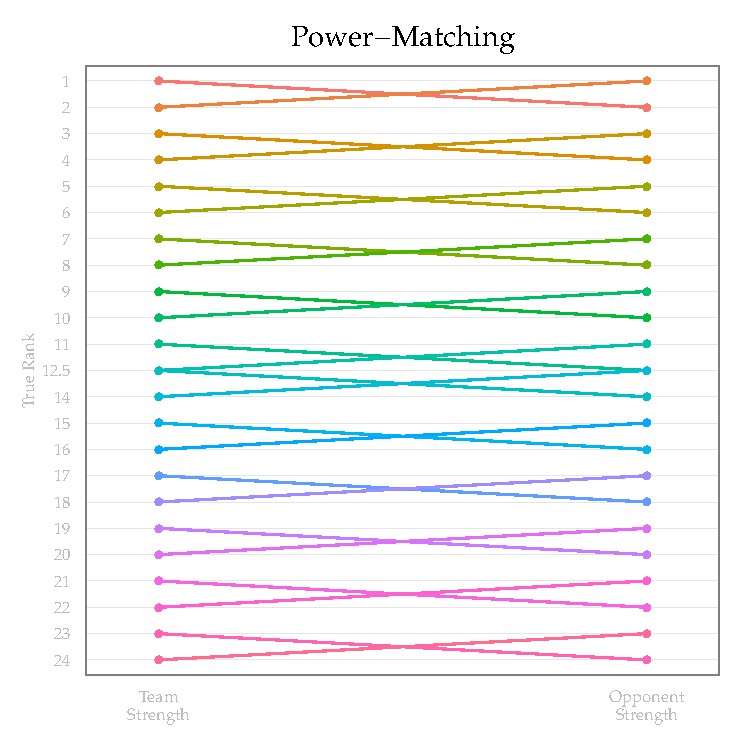
\includegraphics[width=\linewidth]{power-matching_demo.pdf}
  \caption{The strongest team is matched to the next strongest team, etc.}
  \label{fig:demo_power}
\end{marginfigure}

The $n$ teams at a tournament are ranked from 1 to $n$ where 1 represents the strongest team. Teams are paired such that Team 1 faces Team 2, Team 3 faces Team 4 ... Team $n-1$ faces Team $n$, as shown in Figure~\ref{fig:demo_power}. This procedure is the same as power-matching in Rounds 2 through 4.

\subsection{Folding}
\begin{marginfigure}%
  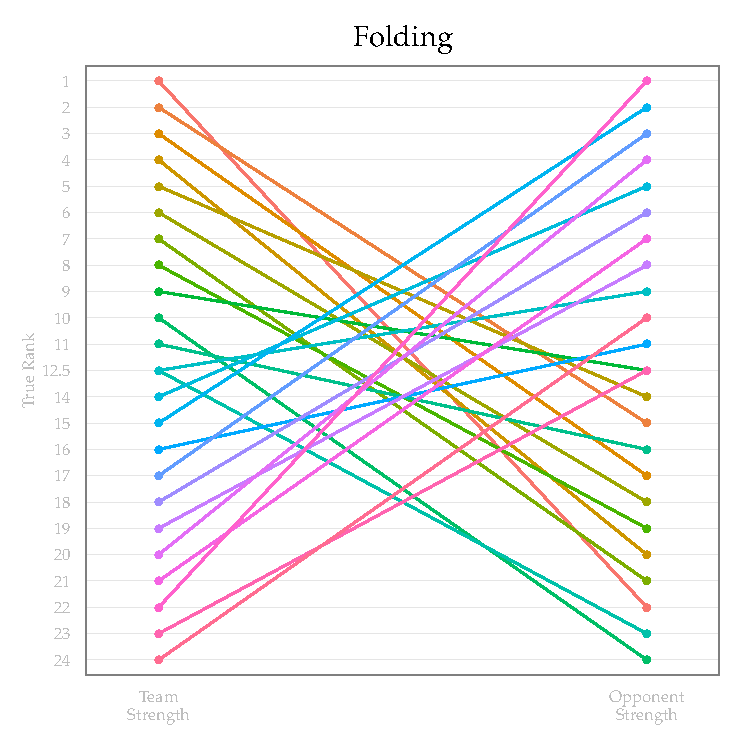
\includegraphics[width=\linewidth]{folding_demo.pdf}
  \caption{Each team in the top twelve is randomly assigned to a team in the bottom twelve. Proposed as Motion Tab-05 by Mike Kelly (UCLA) at the \href{http://www.collegemocktrial.org/2013AMTAagendafinal.pdf}{2013 AMTA Summer Board Meeting}.}
  \label{fig:demo_fold}
\end{marginfigure}

The $n$ teams at a tournament are ranked from 1 to $n$ where 1 represents the strongest team. Teams are separated into two brackets: the `top' group consists of Team 1, Team 2 ...  Team $n/2$ and the `bottom' group consists of Team $n/2 + 1$, Team $n/2 + 2$ ... Team $n$. Each team in the `top' group is randomly paired against a team in the `bottom' group until all teams are paired. Figure~\ref{fig:demo_fold} displays one possible set of Round 1 pairings.

\subsection{Envelope}
\begin{marginfigure}%
  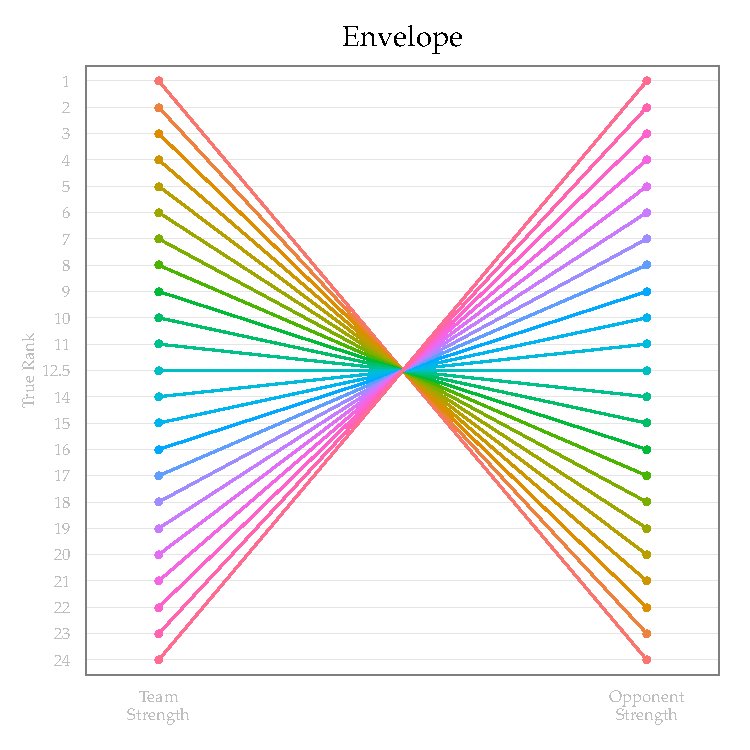
\includegraphics[width=\linewidth]{envelope_demo.pdf}
  \caption{Envelope pairing combines Power and Folding pairing.}
  \label{fig:demo_envel}
\end{marginfigure}
The $n$ teams at a tournament are ranked from 1 to $n$ where 1 represents the strongest team. Teams are ranked such that Team 1 faces Team $n$, Team 2 faces Team $n-1$ ... Team $n/2$ faces Team $n/2 + 1$. Figure~\ref{fig:demo_envel} displays the Round 1 pairing.

\section{Methodology}
We built four simulations of mock trial tournaments: Model A follows standard AMTA procedures and randomly pairs Round 1, Model B uses power ranking for Round 1 pairings, Model C uses the Folding procedure, and Model D uses the Envelope procedure.

For each simulation, we construct a standard 24-team field, and each team is assigned a \emph{true strength} value, which determines the point differential of any round.\marginnote[-2\baselineskip
]{While we considered assigning a variance term to each team's strength, these variations would average to zero over the course of large-$n$ simulations, so we omitted this factor for simplicity. In future work, we plan to test the robustness of our results by adding a variance term to both team strength and judge perception.} That is, if Team A had an assigned strength of 70 and Team B had an assigned strength of 80, the simulated point differential would be -10 (from the perspective of Team A). Because each team's true strength determined the point differential, we only simulate one ballot per round. Using the results of each trial, we pair subsequent rounds using the standard procedures for invitational tournaments with one exception: while we power-match Rounds 2 through 4 and respect side-constraints, our simulation does not take into account impermissible matches, so the same teams may face each other twice in the same tournament. Over a sufficiently large number of simulations, we expect any bias introduced by this element to average to zero. The only component that differed across models was the procedure used to pair Round 1.\marginnote{For the variations in Round 1 pairing that require the teams to be ranked by strength, we rank the teams based on their specified true strength value.}

For each of the four models, we simulate 5,000 tournaments to generate data from 20,000 tournaments in total. In each simulated tournament, the twenty-four teams have the same initial distribution of team strength. To evaluate the results, we compare the the team rankings observed at the conclusion of each simulated tournament to the true team rank, as determined by the true strength specified at the start of each simulated trial. 

To implement the simulations, we use the computing language \emph{R}. Code and replication data are available on request.\marginnote{Please contact \href{mailto:anniejw6@gmail.com}{Annie J. Wang.}}

\section{Results}

To evaluate which system of Round 1 pairing is the most accurate, we are interested in two measures: bias and variance.

\begin{itemize}
\item Bias refers to the expected difference between the predicted outcome and the true outcome. In this case, we compared the team rankings generated by each simulated trial against the true distribution of team strength. All else equal, lower bias is preferred to higher bias. \marginnote[-3\baselineskip
]{For $n$ observations, $$\text{bias} =\frac{1}{n}\sum_{i=1}^{n} (\text{Observed}_i - \text{True}_i)$$}
\item  Variance refers to the \emph{spread} of errors.\marginnote[-1\baselineskip
]{As our measure of variance, we use root mean squared error, which is calculated as $$\text{rmse} = \sqrt{\text{bias}^2}$$} On average (across the entire dataset), a procedure can procedure very accurate results, but variance describes the tendency of any individual result to differ. All else equal, we prefer procedures that lead to lower variance over those that lead to higher variance.
\end{itemize}

Figure~\ref{fig:bias_var} displays the bias and variance of the four pairing systems, averaged across all tournaments and all teams. The bias, represented by the points, is zero for all four systems. That might seem strange, but recall that when we calculate bias, we average errors across all the teams in a tournament. If a ranking system consistently ranks the top team as the worst team (difference between observed and true: -24), as long as it also ranks the worst team as the top team (difference between true and observed: +24), those errors cancel out: the average difference is zero.  \marginnote[-4\baselineskip
]{What kind of ranking system would have a non-zero bias? If the average rank produced by the ranking system were not equal to the average rank based on true team strength, e.g. a ranking system that tied every team.}
\begin{figure}
  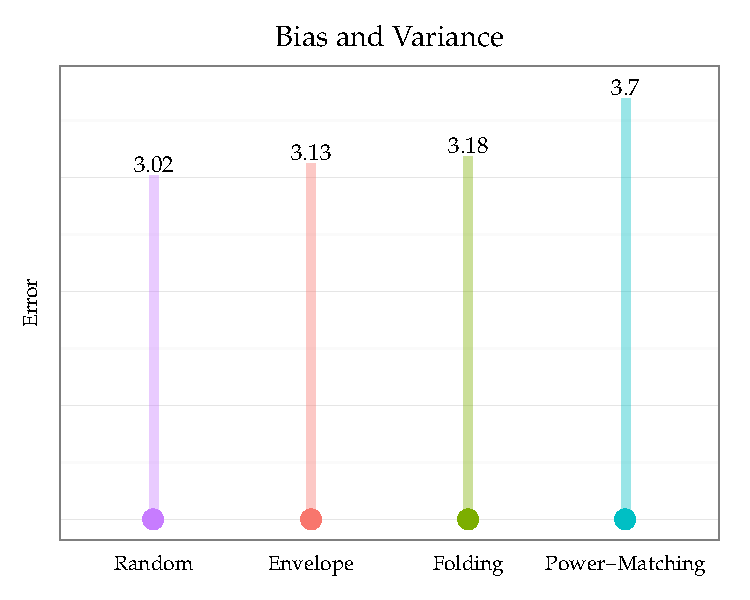
\includegraphics[width=0.7\linewidth]{error_bar.pdf}
%  \checkparity This is an \pageparity\ page.%
  \caption{The average bias of all four systems is zero, and the bars extending upward represent the variance of each pairing system.)}
  \label{fig:bias_var}
  %\zsavepos{pos:textfig}
  \setfloatalignment{b}
\end{figure}

The variances, represented by the vertical bars, are more useful for distinguishing the four pairing systems. We see that the random system has the lowest variance and power-matching the highest. That is, the existing Random pairing system outperforms other methods of pairing Round 1 in terms of accuracy.

For a more granular analysis, Figures~\ref{fig:bias_teamRank}~and~\ref{fig:rmse_teamRank} show bias and variance calculated by the true rank of each team. Here, we see that the Random pairing creates relatively even biases and variance across the teams. By contrast, the Envelope and Power-Matching pairing create highly uneven distributions of bias. Power-matching, in particular, appears to have an alternating pattern of biases: this pattern is explained, at least in part, by the fact that after Round 1, at least half the teams in the top half have a loss from which they need to recover in the rest of the tournament. 

\begin{figure*}[h]
  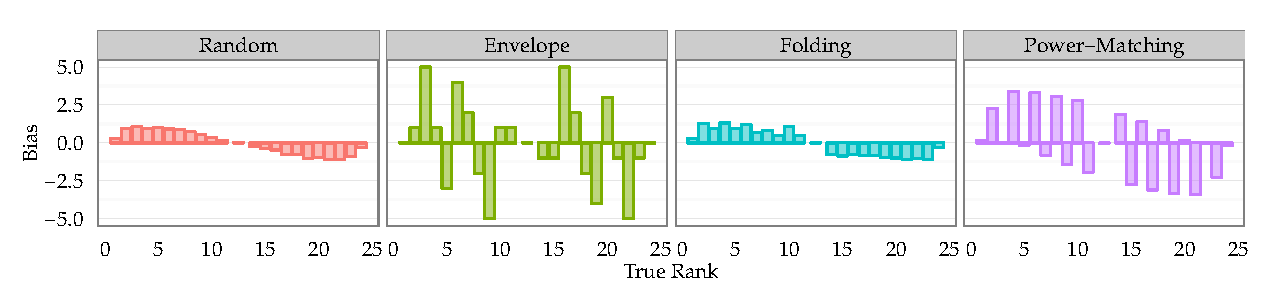
\includegraphics[width=\linewidth]{bias_teamRank.pdf}%
  \caption{Bias by Team Strength}%
  \label{fig:bias_teamRank}%
\end{figure*}

\begin{figure*}[h]
  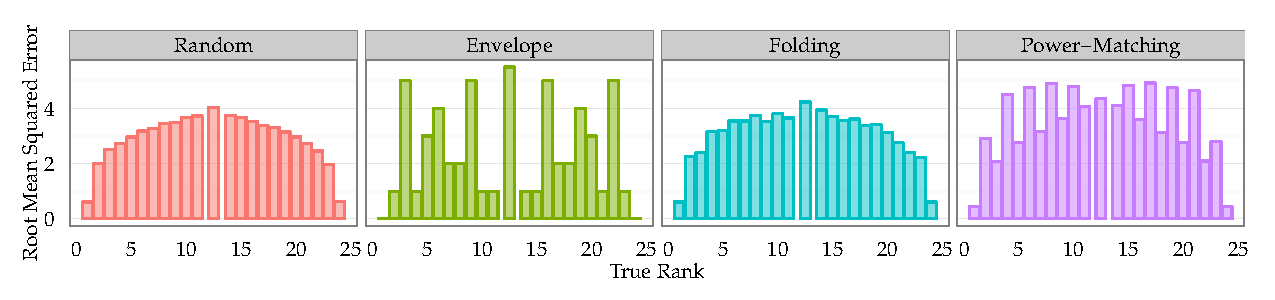
\includegraphics[width=\linewidth]{rmse_teamRank.pdf}%
  \caption{Variance by Team Strength}%
    \label{fig:rmse_teamRank}%
\end{figure*}

Among the four systems, the Folding and Random pairings look the most similar (see Figures~\ref{fig:ranfold_bias}~and~\ref{fig:ranfold_rmse}). This make sense since Folding is essentially a Random pairing with the additional constraint that teams are separated into two halves from the onset. Despite their similarity, Random pairings are less biased than Folding for 12 out of the 23 true ranks and have lower variance for 18 out of the 23 true ranks.\marginnote[-2\baselineskip
]{There are 24 teams in each tournament but only 23 true ranks because the two teams in the middle were assigned equal team strengths and, accordingly, were both ranked 12.5.} 

 
\begin{marginfigure}%
  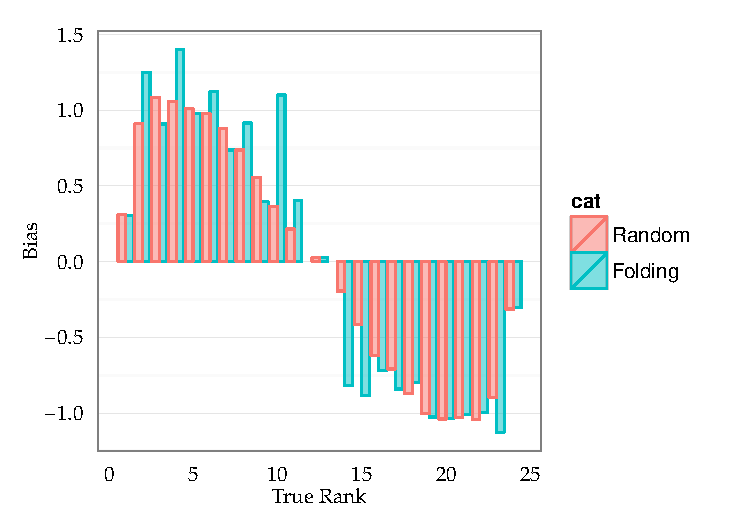
\includegraphics[width=\linewidth]{bias_ranfold.pdf}
  \caption{Bias in Random vs. Folding methods}
  \label{fig:ranfold_bias}
\end{marginfigure}

\begin{marginfigure}%
  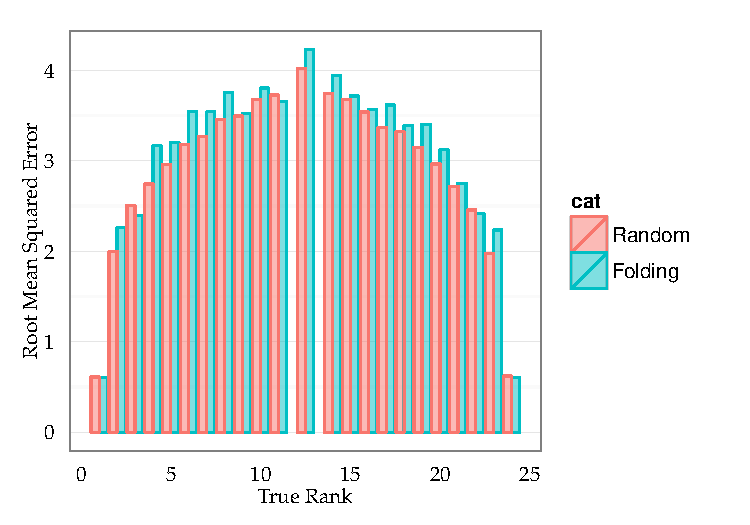
\includegraphics[width=\linewidth]{rmse_ranfold.pdf}
  \caption{Variance in Random vs. Folding methods}
  \label{fig:ranfold_rmse}
\end{marginfigure}

\section{Conclusion and Further Work}
After simulating four different types of Round 1 pairing systems, we find that the existing AMTA random pairing system offers the most accurate results. This result is particularly surprising because we test it against the strongest possible implementation of the other ranking systems: one with perfect information. In practice, it would be extremely difficult to predict the true strength of any team, and although we do not test it here, mistakes in the initial rankings would likely diminish the (theorized) benefits of those pairing systems.

More broadly, this analysis demonstrates the utility of simulations for analyzing proposed changes to tabulation procedure. Going forward, these techniques can be used to analyze almost any component of ranking or pairing methods, such as the impact of power-protecting in Regionals and Opening Round Championships or the utility of new tabulation systems such as \href{http://anniejw.com/WPB/}{Weighted Partial Ballots}. We believe this technique enhances our understanding of the impact of changes in tabulation, and we welcome any suggestions about how to improve these simulations or idea of analyses for which they may prove useful.
\end{document}
